\documentclass[11pt]{article}

\newcommand{\yourname}{Zerun Tian}
\newcommand{\yourcollaborators}{}

\def\comments{0}

%format and packages

%\usepackage{algorithm, algorithmic}
\usepackage[noend]{algpseudocode}
\usepackage{amsmath, amssymb, amsthm}
\usepackage{enumerate}
\usepackage{enumitem}
\usepackage{framed}
\usepackage{verbatim}
\usepackage[margin=1.0in]{geometry}
\usepackage{microtype}
\usepackage{kpfonts}
\usepackage{palatino}
	\DeclareMathAlphabet{\mathtt}{OT1}{cmtt}{m}{n}
	\SetMathAlphabet{\mathtt}{bold}{OT1}{cmtt}{bx}{n}
	\DeclareMathAlphabet{\mathsf}{OT1}{cmss}{m}{n}
	\SetMathAlphabet{\mathsf}{bold}{OT1}{cmss}{bx}{n}
	\renewcommand*\ttdefault{cmtt}
	\renewcommand*\sfdefault{cmss}
	\renewcommand{\baselinestretch}{1.06}
\usepackage[usenames,dvipsnames]{xcolor}
\definecolor{DarkGreen}{rgb}{0.15,0.5,0.15}
\definecolor{DarkRed}{rgb}{0.6,0.2,0.2}
\definecolor{DarkBlue}{rgb}{0.2,0.2,0.6}
\definecolor{DarkPurple}{rgb}{0.4,0.2,0.4}
\usepackage[pdftex]{hyperref}
\hypersetup{
	linktocpage=true,
	colorlinks=true,				% false: boxed links; true: colored links
	linkcolor=DarkBlue,		% color of internal links
	citecolor=DarkBlue,	% color of links to bibliography
	urlcolor=DarkBlue,		% color of external links
}

\usepackage{tikz-qtree}
\tikzset{every tree node/.style={minimum width=2em,draw,circle},
         blank/.style={draw=none},
         edge from parent/.style=
         {draw,edge from parent path={(\tikzparentnode) -- (\tikzchildnode)}},
         level distance=1.5cm}
\usepackage{graphicx}
\graphicspath{ {./} }


%enclosure macros
\newcommand{\paren}[1]{\ensuremath{\left( {#1} \right)}}
\newcommand{\bracket}[1]{\ensuremath{\left\{ {#1} \right\}}}
\renewcommand{\sb}[1]{\ensuremath{\left[ {#1} \right\]}}
\newcommand{\ab}[1]{\ensuremath{\left\langle {#1} \right\rangle}}

%probability macros
\newcommand{\ex}[2]{{\ifx&#1& \mathbb{E} \else \underset{#1}{\mathbb{E}} \fi \left[#2\right]}}
\newcommand{\pr}[2]{{\ifx&#1& \mathbb{P} \else \underset{#1}{\mathbb{P}} \fi \left[#2\right]}}
\newcommand{\var}[2]{{\ifx&#1& \mathrm{Var} \else \underset{#1}{\mathrm{Var}} \fi \left[#2\right]}}

%useful CS macros
\newcommand{\poly}{\mathrm{poly}}
\newcommand{\polylog}{\mathrm{polylog}}
\newcommand{\zo}{\{0,1\}}
\newcommand{\pmo}{\{\pm1\}}
\newcommand{\getsr}{\gets_{\mbox{\tiny R}}}
\newcommand{\card}[1]{\left| #1 \right|}
\newcommand{\set}[1]{\left\{#1\right\}}
\newcommand{\negl}{\mathrm{negl}}
\newcommand{\eps}{\varepsilon}
\DeclareMathOperator*{\argmin}{arg\,min}
\DeclareMathOperator*{\argmax}{arg\,max}
\newcommand{\eqand}{\qquad \textrm{and} \qquad}
\newcommand{\ind}[1]{\mathbb{I}\{#1\}}
\newcommand{\sslash}{\ensuremath{\mathbin{/\mkern-3mu/}}}
\newcommand{\floor}[1]{\left\lfloor #1 \right\rfloor}
\newcommand{\ceil}[1]{\left\lceil #1 \right\rceil}

%mathbb
\newcommand{\N}{\mathbb{N}}
\newcommand{\R}{\mathbb{R}}
\newcommand{\Z}{\mathbb{Z}}
%mathcal
\newcommand{\cA}{\mathcal{A}}
\newcommand{\cB}{\mathcal{B}}
\newcommand{\cC}{\mathcal{C}}
\newcommand{\cD}{\mathcal{D}}
\newcommand{\cE}{\mathcal{E}}
\newcommand{\cF}{\mathcal{F}}
\newcommand{\cL}{\mathcal{L}}
\newcommand{\cM}{\mathcal{M}}
\newcommand{\cO}{\mathcal{O}}
\newcommand{\cP}{\mathcal{P}}
\newcommand{\cQ}{\mathcal{Q}}
\newcommand{\cR}{\mathcal{R}}
\newcommand{\cS}{\mathcal{S}}
\newcommand{\cU}{\mathcal{U}}
\newcommand{\cV}{\mathcal{V}}
\newcommand{\cW}{\mathcal{W}}
\newcommand{\cX}{\mathcal{X}}
\newcommand{\cY}{\mathcal{Y}}
\newcommand{\cZ}{\mathcal{Z}}

%theorem macros
\newtheorem{thm}{Theorem}
\newtheorem{lem}[thm]{Lemma}
\newtheorem{fact}[thm]{Fact}
\newtheorem{clm}[thm]{Claim}
\newtheorem{rem}[thm]{Remark}
\newtheorem{coro}[thm]{Corollary}
\newtheorem{prop}[thm]{Proposition}
\newtheorem{conj}[thm]{Conjecture}

\theoremstyle{definition}
\newtheorem{defn}[thm]{Definition}


\newcommand{\instructor}{Virgil Pavlu}
\newcommand{\hwnum}{2A}
\newcommand{\hwdue}{\href{https://gradescope.com/courses/229309}{Gradescope}}

\theoremstyle{theorem}
\newtheorem{prob}{}
\newtheorem{sol}{Solution}

\definecolor{cit}{rgb}{0.05,0.2,0.45} 
\newcommand{\solution}{\medskip\noindent{\color{DarkBlue}\textbf{Solution:}}}

\begin{document}
{\Large 
\begin{center}{CS5800: Algorithms} --- Spring '21 --- \instructor \end{center}}
{\large
\vspace{10pt}
\noindent Homework~\hwnum \vspace{2pt}\\
Due :~\hwdue}

\bigskip
{\large \noindent Name: \yourname }

\vspace{15pt}

{\large \noindent Instructions:}

\begin{itemize}

\item Make sure to put your name on the first page.  If you are using the \LaTeX~template we provided, then you can make sure it appears by filling in the \texttt{yourname} command.

\item Please review the grading policy outlined in the course information page.

\item You must also write down with whom you worked on the assignment.  If this changes from problem to problem, then you should write down this information separately with each problem.

\item Problem numbers (like Exercise 3.1-1) are corresponding to CLRS $3^{rd}$ edition.  While the  $2^{nd}$ edition  has  similar  problems  with  similar  numbers,  the  actual  exercises  and their solutions are different, so make sure you are using the $3^{rd}$ edition.

\end{itemize}

\newpage

%%% Problem 1 %%%
\begin{prob} \textbf{(5 points)} Exercise 6.1-4, explain why.

Where in a max-heap might the smallest element reside, assuming that all elements are distinct?

\solution

In the tree representation of a max-heap, the smallest element resides in one of the leaf nodes. In the array representation, the smallest element appears in $A[\floor{n/2} + 1:]$, from index $\floor{n/2}+1$ to the last index (inclusion). We can prove this by contradiction. Let's assume that the smallest element exists in a non-leaf node. Because all elements are distinct, the values in children of the non-leaf node, containing the smallest value, must be greater, which breaks the max-heap property. Our assumption leads to an invalid max-heap, so we showed that the smallest element resides in a leaf node.
\end{prob}

\newpage
%%% Problem 2 %%%
\begin{prob} \textbf{(5 points)} Exercise 6.1-6, explain why.

Is the array with values $[23, 17, 14, 6, 13, 10, 1, 5, 7, 12]$ a max-heap?

\solution

Drawing the corresponding tree of the above values, we can easily spot any problems.

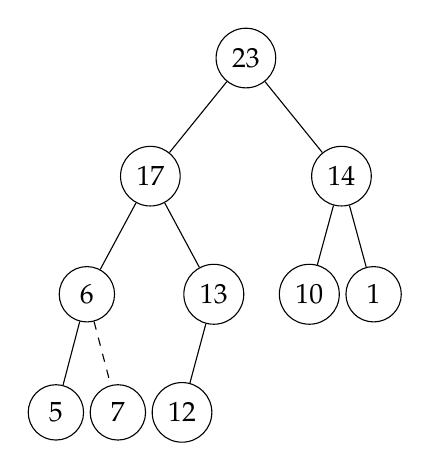
\begin{tikzpicture}
\Tree
[.23     
	[.17 
        		[.6
        			5
        			\edge[dashed]; {7}
        		]
    		[.13
    			12
			\edge[blank]; \node[blank]{};
    		]
    	]
    	[.14 
    		10
    		1
    	]
]
\end{tikzpicture}

We notice that the node with value 6 is smaller than the right child with value 7. This break the max-heap property, so it's not a max-heap.
\end{prob}

\newpage
%%% Problem 3 %%%
\begin{prob} \textbf{(10 points)} Exercise 6.2-1.

Illustrate the operation of $\text{MAX-HEAPIFY(A, 3)}$ on the array $A = [27, 17, 3, 16, 13, 10, 1, 5, 7, 12, 4, 8, 9, 0]$.

\solution

\includegraphics[scale=0.7]{hw2q3.png}

In the initial configuration (a), the node at index 3 has value 3 which is not greater than its direct left child of value 10. In (b), we exchange the value 10 with 3. Then, it enters the recursive call, which compares 3 with direct children out of which the right child has a greater value of 9. Performing the same exchange operation, we end up with the configuration (c) which terminates.
\end{prob}

\newpage
%%% Problem 4 %%%
\begin{prob} \textbf{(10 points)} Exercise 6.3-1.

Illustrate the operation of $\text{BUILD-MAX-HEAP}$ on the array $A = [5, 3, 17, 10, 84, 19, 6, 22, 9]$.

\solution

\includegraphics[scale=0.65]{hw2q4.png}

In the initial configuration (a), we start from the gray node of value 10. It compares with its direct children among which the left child of value 22 is greater. The value 10 is swapped with 22, and we move on to the next gray node of value 17. In configuration (b), we find 17 is not greater than its direct left child 19, running $\text{MAX-HEAPIFY}$ results in (c). In the next iteration, the gray node of value 3 is less than both children, among which the right child of value 84 is larger, which results in (d). In (e), the gray node of value 5 is not greater its left child 22. Running $\text{MAX-HEAPIFY}$ results in (f). Finally, the max-heap is built completely after the value 5 is swapped with 10 which is greater. 
\end{prob}

\newpage
%%% Problem 5 %%%
\begin{prob} \textbf{(15 points)} Problem 6-2.

\begin{enumerate}
%%% Problem 5.1 %%%
\item How would you represent a d-ary heap in an array?

\solution

Suppose we are using 1-based indexing. To find the k-th child of the element i, we can compute $(i-1)d + k +1$ to get its exact index in the array. The parent of the child $i$ can be found using the formula, $\floor{(i-2+d)/d}$. As such, we can represent the parent-child relationship of a d-ary heap in an array.

%%% Problem 5.2 %%%
\item What is the height of a d-ary heap of n elements in terms of n and d?

\solution

Suppose that the heap is full, meaning the last layer of the tree is filled with leaves. The total number of nodes in the heap, $n$, can be written as a geometric series. We know the sum of such sequence can be calculated using the closed-form formula --- $(1-d^k) / (1-d)$ where $k$ is the number of layers of the tree. The height of the tree is just $k-1$. Let's solve k,
\[
\begin{split}
\frac{1-d^k}{1-d} &= n \\
1-d^k &= n - dn \\
d^k &= dn - n + 1 \\
k &= \log_d^{dn - n + 1}
\end{split}
\]
The height of such heap is $\log_d^{dn - n + 1} - 1 = \log_d^{n - n/d + 1/d}$. On the other hand, the last layer of the same height tree can contain as little as one leaf (all other leaf nodes are one-layer above). In this case, we can express $n$ to be $(1-d^{k-1})/(1-d) + 1$.
\[
\begin{split}
\frac{1- d^{k-1}}{1-d} + 1 &= n \\
\frac{1- d^{k-1}}{1-d} &= n - 1 \\
1 - d^{k-1} &= n - dn - 1 + d \\
d^{k-1} &= dn - n + 2 - d \\
k-1 &= \log_d^{dn - n + 2 - d} \\
\end{split}
\]
In this case, the height is $\log_d^{dn - n + 2 - d}$. We observe that the height of the tree is bounded by $\log_d^n$.

\newpage
%%% Problem 5.3 %%%
\item Give an efficient implementation of EXTRACT-MAX in a d-ary max-heap. Analyze its running time in terms of d and n.

\solution

Suppose we are working with 1-based indexing. Before we start, let's define two primitive helper functions $\textproc{\textsc{Parent}}$ and $\textproc{\textsc{Child}}$ using the answer to problem 5.1.

\begin{algorithmic}[1]
\Function{Parent}{i}
	\State \textbf{return} floor$((i-2+d)/d)$
\EndFunction
\end{algorithmic}

\begin{algorithmic}[1]
\Function{Child}{i, k} \Comment{the k-th child of node i}
	\State \textbf{return} $(i-1)d + k + 1$
\EndFunction
\end{algorithmic}

The $\textproc{\textsc{ExtractMax}}$ function is exactly the same as it is for the binary heap.

\begin{algorithmic}[1]
\Function{ExtractMax}{$A$}
	\If {$A.\text{heap-size} < 1$}
		\State \textbf{throw} error "heap underflow"
	\EndIf
	\State $\textit{max} = A[1]$
	\State $A[1] = A[A.\text{heap-size}]$
	\State $A.\text{heap-size} = A.\text{heap-size} - 1$
	\State $\textproc{\textsc{MaxHeapify}}(A, 1)$
	\State \textbf{return} $\textit{max}$
\EndFunction
\end{algorithmic}

What differs is the $\textproc{\textsc{MaxHeapify}}$ function.

\begin{algorithmic}[1]
\Function{MaxHeapify}{$A$, $i$}
	\State largest $= i$
	\For {$k=1$, $k<=d$, $\textit{k++}$} \Comment{find a child that has the largest value}
		\State child $= \textproc{\textsc{Child}}(A, i, k)$
		\If {$child \le A.\text{heap-size}$ and $A[\text{child}] > A[\text{largest}]$}
			\State largest = child
		\EndIf
	\EndFor
	\If {largest $\neq$ i} \Comment{swap the largest child with the value of the current node i}
		\State tmp $= A[\text{largest}]$
		\State $A[\text{largest}] = A[i]$
		\State $A[i] = \text{tmp}$
		\State $\textproc{\textsc{MaxHeapify}}$(A, largest) \Comment{call recursively on the node being updated}
	\EndIf
\EndFunction
\end{algorithmic}
For the $\textproc{\textsc{MaxHeapify}}$ function, the depth of the recursion is at most the height of the heap, which is bounded by $\log_d^n$. In every call, constant amount of work are executed d times in the for loop at line 3. In total, the running time is $O(d\log_d^n)$.

\newpage
%%% Problem 5.4 %%%
\item Give an efficient implementation of INSERT in a d-ary max-heap. Analyze its running time in terms of d and n.

\solution

\begin{algorithmic}[1]
\Function{Insert}{$A$, $val$}
	\State $A.\text{heap-size} = A.\text{heap-size} + 1$ \Comment{create a leaf and add the value there}
	\State $A[A.\text{heap-size}] = val$
	\State $i = A.\text{heap-size}$
	\While {$i > 1$ and $A[\textproc{\textsc{Parent}}(i)] < A[i]$} \Comment{move the node i up if it's greater than its parent}
		\State tmp $= A[i]$
		\State $A[i] = A[\textproc{\textsc{Parent}}(i)]$
		\State $A[\textproc{\textsc{Parent}}(i)] = tmp$ 
		\State $i = \textproc{\textsc{Parent}}(i)$
	\EndWhile
\EndFunction
\end{algorithmic}
Operations prior to the while loop takes constant time. What's inside the while loop take constant time, and the loop executes at most "the height of the heap" times. Thus, the running time is $O(\log_d^n)$.

%%% Problem 5.5 %%%
\item Give an efficient implementation of $\text{INCREASE-KEY(A, i, k)}$, which flags an error if $k < A[i]$, but otherwise sets $A[i] = k$ and then updates the d-ary max-heap structure appropriately. Analyze its running time in terms of d and n.

\solution

\begin{algorithmic}[1]
\Function{IncreaseKey}{$A$, $i$, $k$}
	\If {$k < A[i]$}
		\State \textbf{throw} error "the new value k is not greater than the current value"
	\EndIf
	\State $A[i] = k$
	\While {$i > 1$ and $A[\textproc{\textsc{Parent}}(i)] < A[i]$} 		
		\State tmp $= A[i]$
		\State $A[i] = A[\textproc{\textsc{Parent}}(i)]$
		\State $A[\textproc{\textsc{Parent}}(i)] = tmp$ 
		\State $i = \textproc{\textsc{Parent}}(i)$
	\EndWhile
\EndFunction
\end{algorithmic}
Similar to the last problem, operations prior to the while loop takes constant time. What's inside the loop takes constant time, and the loop executes at most $\log_d^n$ times, which is the depth of the heap. Thus, the running time is $O(\log_d^n)$.

\end{enumerate}
\end{prob}

\newpage
%%% Problem 6 %%%
\begin{prob} \textbf{(5 points)} Exercise 7.2-1.

Use the substitution method to prove that the recurrence $T(n) = T(n-1) + \Theta{(n)}$ has the solution $T(n) = \Theta{(n^2)}$, as claimed at the beginning of Section 7.2.

\solution

We want to show that $c_1 n^2 \leq T(n) \leq c_2 n^2$. 

- First, let's prove the lower bound $T(n) \ge c_1 n^2$ via induction. 

Let's make an inductive hypothesis, $T(n-1) \ge c_1(n-1)^2$.
\[
\begin{split}
T(n) &= T(n-1) + \Theta{(n)} \\
& \ge c_1(n-1)^2 + c_3 n \\
&= c_1 n^2 - 2 c_1 n + c_1 + c_3 n \\
&= c_1 n^2 - (2c_1 - c_3)n + c_1
\end{split}
\]

We want the expanded expression to be greater than or equal to $c_1n^2$,
\[
\begin{split}
T(n) \ge c_1 n^2 - (2c_1 - c_3)n + c_1 &\stackrel{?}{\ge} c_1 n^2 \\
(c_3 - 2c_1)n + c_1 &\stackrel{?}{\ge} 0
\end{split}
\]

We can choose $c_1 = 1$ and $c_3 = 2$, so we have $1 \ge 0$. The lower bound is proved to be correct via induction.

- Second, let's show the upper bound $T(n) \leq c_2 n^2$ is correct.

Let's make an inductive hypothesis, $T(n-1) \leq c_2 (n-1)^2$.
\[
\begin{split}
T(n) &= T(n-1) + \Theta{(n)} \\
& \leq c_2 (n-1)^2 + c_4 n \\
&= c_2 n^2 - 2 c_2 n + c_2 + c_4 n \\
&= c_2 n^2 - (2c_2 - c_4)n + c_2
\end{split}
\]

We want the expression to be less than or equal to $c_2 n^2$,
\[
\begin{split}
T(n) \leq c_2 n^2 - (2c_2 - c_4)n + c_2 &\stackrel{?}{\leq} c_2 n^2 \\
(c_4 - 2c_2)n + c_2 &\stackrel{?}{\leq} 0 \\
c_2 &\stackrel{?}{\leq} (2c_2 - c_4)n \\
\end{split}
\]

Based on the above inequality, we can choose $c_2$, $c_4$ such that $2 c_2 \ge c_4$ and $n \ge c_2/(2c_2 - c_4)$. Let's choose $c_2 = 1$ and $c_4 = 1$. Plugging them into the equation, we have $1 \leq n$. Since $n$ could be arbitrarily large, we proved the upper bound is correct by induction. Thus, $T(n) = \Theta{(n^2)}$.
\end{prob}

\newpage
%%% Problem 7 %%%
\begin{prob} \textbf{(5 points)} Exercise 7.2-2, explain why.

What is the running time of $\text{QUICKSORT}$ when all elements of array $A$ have the same value?

\solution

When all elements are the same, the partition is unbalanced at every recursive call in which one partition has zero element, and the other has the rest. This is the worst case scenario for quicksort described in the page 175 of the CLRS book. The corresponding recurrence is $T(n) = T(n-1) + T(0) + \Theta{(n)} = T(n-1) + \Theta{(n)}$, which has been shown to be quadratic $T(n) = \Theta{(n^2)}$ in problem 6.
\end{prob}

\newpage
%%% Problem 8 %%%
\begin{prob} \textbf{(5 points)} Exercise 7.2-3.

Show that the running time of QUICKSORT is $\Theta{(n^2)}$ when the array $A$ contains distinct elements and is sorted in decreasing order.

\solution

In quicksort, elements are shuffled into partitions. Let's say the elements smaller than or equal to the pivot are in the "small" partition, and the elements greater than pivot are in the "big" partition for the sake of simplicity.

The pivot is selected as the right most element bounded by the left and right indices in each recursive call. From the beginning, because the array is already sorted in descending order, elements from the left are all greater than the pivot, so the "small" partition has size 0 and the "big" partition has size $n-1$. The pivot (the smallest value) will be swapped with the first element of the "big" partition (the largest value). In the next call, the new pivot ends up being the largest value of the array. Again, the partition is extremely unbalanced with the "small" partition of size $n-2$ and the "big" partition of size 0. 

So on so forth, we realize that the partition is always unbalanced. Similar to problem 7, the recurrence is $T(n) = T(n-1) + T(0) + \Theta{(n)} = T(n-1) + \Theta{(n)}$, which has been shown to be quadratic $T(n) = \Theta{(n^2)}$ in problem 6.
\end{prob}

\newpage
%%% Problem 9 %%%
\begin{prob} \textbf{(15 points)} Exercise 7.4-1.

Show that in the recurrence
$T(n) = \underset{0 \leq q \leq n-1}{max} (T(q) + T(n-q-1)) + \Theta{(n)}$, $T(n) = \Omega{(n^2)}$.

\solution

Similar to how the book (CLRS 7.4.1) proved the upper bound - $O(n^2)$, the worst-case running time of the recurrence of quicksort, we can prove the lower bound $\Omega{(n^2)}$ using the substitution method.

Let's make a strong inductive hypothesis that $T(m) \ge c m^2$ for all $m < n$. Substituting this hypothesis into the recurrence above, we have,
\[
\begin{split}
T(n) &= \underset{0 \leq q \leq n-1}{max} (T(q) + T(n-q-1)) + \Theta{(n)} \\
&\ge \underset{0 \leq q \leq n-1}{max} (cq^2 + c(n-q-1)^2) + \Theta{(n)} \\
&= c \cdot \underset{0 \leq q \leq n-1}{max} (q^2 + (n-q-1)^2) + \Theta{(n)}
\end{split}
\]
Let's find the parameter $q$ that let the expression $f(n, q) = q^2 + (n-q-1)^2$ achieve a maximum.
\[
\begin{split}
f(n, q) = q^2 + (n-q-1)^2 &= q^2 + n^2 - nq -n - nq + q^2 + q - n + q + 1 \\
&= n^2 + 2q^2 - 2nq - 2n + 2q + 1
\end{split}
\]
The first derivative w.r.t. $q$ is $\frac{\partial f}{\partial q} = 4q - 2n + 2$. The second derivative w.r.t. $q$ is that $\frac{\partial^2 f}{\partial q^2} = 4$, which is positive. This tells us that a maximum can be found at either endpoint of the bound. Plugging either $q = 0$ or $q = n-1$ into $f(n, q)$, we have $(n-1)^2$. This tells us that $\underset{0 \leq q \leq n-1}{max} (q^2 + (n-q-1)^2) = (n-1)^2 = n^2 - 2n + 1$. Let's substitute that back to the recurrence,
\[
\begin{split}
T(n) &\ge c \cdot \underset{0 \leq q \leq n-1}{max} (q^2 + (n-q-1)^2) + \Theta{(n)} \\
&= c (n^2 - 2n + 1) + \Theta{(n)} \\
&= c n^2 - c(2n - 1) + \Theta{(n)} \\
&\stackrel{?}{\ge} cn^2 
\end{split}
\]
We want $c n^2 - c(2n - 1) + \Theta{(n)} \stackrel{?}{\ge} cn^2$, so simplifying it, 
\[
\begin{split}
- c(2n - 1) + \Theta{(n)} &\stackrel{?}{\ge} 0 \\
-2nc + c + c_1 n &\stackrel{?}{\ge} 0
\end{split}
\]
We can choose $c = 1$ and $c_1 = 2$, which gives us $-2n + 1 + 2n = 1 \ge 0$. We successfully showed that $T(n) \ge c n^2$, then we know $T(n) = \Omega{(n^2)}$.
\end{prob} 

\newpage
%%% Problem 10 %%%
\begin{prob} \textbf{(15 points)} Exercise 7.4-2.

Show that quicksort’s best-case running time is $\Omega{(n\lg n)}$.

\solution

On the contrary to its worst-case's recurrence, quicksort's best-case can be written as,
\[
T(n) = \underset{0 \leq q \leq n-1}{min} (T(q) + T(n-q-1)) + \Theta{(n)}
\]
Let's prove this using the substitution method. We make a hypothesis that $T(m) \ge c(m\lg m + 2m)$ for all $m < n$ and some constant $c$. Substituting that back into the recurrence, we get,
\[
\begin{split}
T(n) &= \underset{0 \leq q \leq n-1}{min} (T(q) + T(n-q-1)) + \Theta{(n)} \\
& \ge \underset{0 \leq q \leq n-1}{min} (c (q\lg q + 2q) + c ((n-q-1) \lg (n-q-1) + 2 (n-q-1))) + \Theta{(n)} \\
& = c \cdot \underset{0 \leq q \leq n-1}{min} (q\lg q + 2q + (n-q-1) \lg (n-q-1) + 2 (n-q-1)) + \Theta{(n)} \\
\end{split}
\]
Let's find a minimum of the function $f(n, q) = q\lg q + 2q + (n-q-1) \lg (n-q-1) + 2 (n-q-1)$ by taking the first derivative and set to 0.
\[
\begin{split}
\frac{\partial f}{\partial q} &= 1 \cdot \lg q + q \cdot \frac{1}{\ln 2} \cdot \frac{1}{q} + 2 - \lg(n-q-1) - (n-q-1) \cdot  \frac{1}{\ln 2} \cdot \frac{1}{n-q-1} - 2 \\
& = \lg q + \frac{1}{\ln 2} + 2 - \lg(n-q-1) - \frac{1}{\ln 2} - 2 \\
& = \lg q - \lg(n-q-1)
\end{split}
\]
Setting the first derivative to 0, we have,
\[
\begin{split}
\lg q - \lg(n-q-1) &= 0 \\
\lg \frac{q}{n-q-1} &= 0 \\
 \frac{q}{n-q-1} &= 1 \\
 q &= n - q - 1 \\
 q &= \frac{n-1}{2}
\end{split}
\]
The function $f(n, q)$ reaches a minimum when $q = (n-1)/2$. Substituting q, we have,
\[
\begin{split}
T(n) &= c \cdot \underset{0 \leq q \leq n-1}{min} (q\lg q + 2q + (n-q-1) \lg (n-q-1) + 2 (n-q-1)) + \Theta{(n)} \\
&= c (\frac{n-1}{2} \lg \frac{n-1}{2} + n - 1 + \frac{n-1}{2} \lg \frac{n-1}{2} + n - 1) + \Theta{(n)} \\
&= c ((n-1)\lg \frac{n-1}{2} + 2n - 2) + \Theta{(n)} \\
&= c ((n-1) \cdot (\lg (n-1) - 1) + 2n - 2) + \Theta{(n)} = c ((n-1) \lg (n-1) + n - 1) + \Theta{(n)} \\
&= c(n-1)\lg(n-1) + cn - c + \Theta{(n)} = cn (\lg(n-1) + 1) - c\lg(n-1) - c + \Theta{(n)} \\
&= cn\lg (2n - 2) - c\lg(n-1) - c + \Theta{(n)} \stackrel{?}{\ge} cn\lg n
\end{split}
\]
If we pick a $c$ that is large enough and for a large n, $cn\lg (2n - 2)$ term dominates $- c\lg(n-1) - c + \Theta{(n)}$. We showed $T(n) = \Omega{(n\lg n)}$. Thus, quicksort's best-case running time is $\Omega{(n\lg n)}$.
\end{prob}

\newpage
%%% Problem 11 %%%
\begin{prob} \textbf{(10 points)} Exercise 7.4-3.

Show that the expression $q^2 + (n-q-1)^2$ achieves a maximum over $q = 0,1,\cdots,n-1$ when $q = 0$ or $q = n - 1$.

\solution

To find a maximum of the expression, we first check the sign of the second derivative.
\[
\begin{split}
f(n, q) = q^2 + (n-q-1)^2 &= q^2 + n^2 - nq -n - nq + q^2 + q - n + q + 1 \\
&= n^2 + 2q^2 - 2nq - 2n + 2q + 1
\end{split}
\]
The first derivative w.r.t. $q$ is that $\frac{\partial f}{\partial q} = 4q - 2n + 2$. The second derivative w.r.t. $q$ is that $\frac{\partial^2 f}{\partial q^2} = 4$, which is positive. This means that a critical point will be a minimum, and more importantly, either endpoint of the bound will be a maximum. When $q=0$, the expression becomes $(n-1)^2$, and when $q=n-1$, the expression is also $(n-1)^2$. Thus, when $q=0$ or $q=n-1$, the expression reaches a maximum.
\end{prob}

\newpage
%%% Problem 12 EC %%%
\begin{prob} \textbf{(Extra credit 10 points)} Problem 6-3.
\end{prob}

\end{document}